\label{sec:results}
The qualification tests follow the six requirements of the Project Proposal in order of importance. The physical reproduction, photographed-page analysis and embedded timing records are kept identifiable so that each result can be traced to the part of the system that produced it. Section~\ref{sec:discussion} interprets the engineering consequences; this section states the procedures and measurements.

\subsection{Summary of results achieved}
\label{sec:res-summary}
Table~\ref{tab:res-summary} compares the proposal's intended functions and numerical specifications with the available measurements. A result above a numerical target is distinguished from a complete qualification of the corresponding requirement.

\begin{table}[!htbp]\centering\small
\setlength{\tabcolsep}{5pt}
\begin{tabular}{p{0.32\linewidth}p{0.48\linewidth}p{0.12\linewidth}}\toprule
\textbf{Intended outcome} & \textbf{Actual outcome} & \textbf{Location}\\\midrule
\textbf{R1.} Reproduce any desired digital text in a trained writer's style, with at least 85\% character accuracy and 85\% stylistic correlation. & Fourteen physical pages, 184 labelled lines and 5\,471 reference characters give 84.41\% read-back character accuracy. Seven of eleven writers individually exceed 85\%. Writer identification is 86.41\% by line and all fourteen page pools are correctly attributed. A new geometric comparison of the physical output with 156 original lines gives shape correlation 0.697, below 0.85. The two pooled targets are not met; the writer breakdown identifies demonstrated stronger cases. & QT~1; Appendix~\ref{app:res-evidence}\\[5pt]
\textbf{R2.} Decode handwritten content and identify its writer from the training set with 95\% overall accuracy. & Writer identification reaches 153/156 lines, 98.08\%, and 11/11 writer pools. The selected joint reader reaches 94.06\% character accuracy on 1\,076 validation lines; the numerical comparison reader reaches 94.39\%. The writer point estimate exceeds 95\%; the selected reader is 0.94 percentage points below it. A joint text-and-writer success rate is not inferred from these different populations. & QT~2\\[5pt]
\textbf{R3.} Reproduce desired text in a trained style at no slower than 4~s per character. & \textbf{Met on the completion-confirmed timing records.} All 25 positive-character ODROID records with an explicit program-end marker satisfy their allowances. The worst is 166.61~s for 43 characters, or 3.875~s per character. & QT~3\\[5pt]
\bottomrule\end{tabular}
\caption{Summary of results achieved against the Project Proposal.}\label{tab:res-summary}
\end{table}

\begin{table}[!htbp]\ContinuedFloat\centering\small
\setlength{\tabcolsep}{5pt}
\begin{tabular}{p{0.32\linewidth}p{0.48\linewidth}p{0.12\linewidth}}\toprule
\textbf{Intended outcome} & \textbf{Actual outcome} & \textbf{Location}\\\midrule
\textbf{R4.} Decode the text and identify its writer within $2+0.025x$~s for $x$ handwritten characters. & Two recorded ODROID requests take 46.26~s and 55.49~s, against logged-count allowances of 14.50~s and 26.55~s. \textbf{Not met on these requests.} A separate development-host experiment measures a 2.76-fold network speed improvement using batched library inference. & QT~4\\[5pt]
\textbf{R5.} Draw character trajectories while maintaining absolute positional error no greater than 0.5~mm. & All seven measured square/triangle feature lengths differ from nominal by less than 0.5~mm; the largest difference is 0.37~mm. This supports the calibrated dimensional accuracy. Absolute point-position error and repeated-word overlay performance are not fully qualified by feature lengths alone. & QT~5\\[5pt]
\textbf{R6.} Train at least ten writing styles and permanently store their character trajectory mappings. & \textbf{Met in the evaluated stored set.} Eleven writer identities have stored profiles and glyph mappings and are represented in the evaluated classifier. All eleven are exercised by the physical-output and writer-identification measurements. & QT~6\\[5pt]
\textbf{FC1.} Operate in a well-lit laboratory or office at 400--1000~lux. & Indoor camera captures and robot-page photographs demonstrate operation under the recorded capture conditions. No calibrated illuminance series establishes the complete 400--1000~lux range. & Sec.~\ref{sec:res-conditions}\\[5pt]
\textbf{FC2.} Operate on a stable, level, vibration-free surface. & The physical outputs demonstrate operation in the fixed test arrangement. Surface level and vibration are not quantified, so the evidence applies to that arrangement. & Sec.~\ref{sec:res-conditions}\\
\bottomrule\end{tabular}
\caption{Summary of results achieved against the Project Proposal (continued).}
\end{table}
\FloatBarrier

\subsection{Qualification tests}
\label{sec:res-qtp}
\subsubsection{Test material, configuration and measurement definitions}
\label{sec:res-method}
The final evaluation uses six IAM writers (150, 152, 153, 384, 552 and 588) and five photographed contributors, denoted A, B, O, T and Y. These are the eleven writers introduced in Section~\ref{sec:des-class}. The robot drew fourteen pages because some writers' text occupies two pages. The pages contain a common paragraph, a pangram and, where available, text from the writer's source material. The analysis contains 184 lines with corresponding transcripts; the writer-model comparison additionally evaluates one unpaired crop and therefore contains 185 crops.

The physical pages were produced by the gantry under ODROID control. Accuracy was subsequently scored from saved images on the development host. The embedded timing measurements were extracted from the preserved ODROID server log. This arrangement allows large image sets to be analysed while retaining actual on-device evidence for the time specifications. Numerical equivalence across processors is not assumed to be a new hardware accuracy test.

The reproduction read-back uses the joint reader used in the Design examples. The separate reader evaluation compares that reader with the evaluated scratch reader; the selected joint reader supplies the 94.06\% system result and the scratch reader supplies a 94.39\% comparison result. Both share the architecture in Section~\ref{sec:des-class}. Writer identification uses the eleven-class stroke-normalised classifier at the selected width of 0.17. Appendix~\ref{app:res-evidence} identifies the files by their content hashes, so checkpoints with the same filename cannot be confused.

Character accuracy is computed from the summed Levenshtein edit distance rather than by averaging percentages of unequal-length lines. With reference transcript $t_i$, recognised transcript $\hat t_i$ and distance $d_{\rm edit}$, the scoring definition follows the character-error convention used in handwriting recognition~\cite[p.~2]{graves2006}:
\begin{equation}
A_c=100\left(1-\frac{\sum_i d_{\rm edit}(\hat t_i,t_i)}{\sum_i|t_i|}\right).
\label{eq:res-char}
\end{equation}
For the physical pages, Equation~\ref{eq:res-char} gives $100(1-853/5471)=84.4087\%$. The selected reader gives $100(1-2719/45747)=94.0564\%$, while the numerical reader gives $100(1-2567/45747)=94.3887\%$. Insertions, deletions and substitutions all contribute to the numerator; the score is therefore not a binomial count of independently correct characters.

Writer identification is the number of correctly classified lines divided by the number evaluated. Pooled writer decisions aggregate the evidence from a group of lines and are reported separately. The archive's word score counts matching words at equal positions, divided by reference words; it is called \emph{word match} here. A word insertion can shift later positions, so this score must not be interpreted as one minus word edit error rate.

The measurement tools save transcripts, reference lengths, edit counts and predictions before aggregation. The reviewed tables and figures are regenerated from these saved records. Statistical intervals on line classifications use Wilson score intervals~\cite[pp.~209--212]{wilson1927}; because lines from one writer share writing and capture conditions, these are descriptive line-level intervals. Resampling whole writer groups gives an additional sensitivity check for the physical character score. Neither procedure creates additional independent writers.

\reportqt{qt:r1}{Reproduction of digital text in a trained writer's style (R1)}
\resstep{Objectives of the test or experiment}
Determine whether the complete image-to-profile-to-gantry system produces legible new text in the selected stored style. Evaluate the proposal's character target and distinguish measured geometric style similarity from the supplementary ability to identify the writer of the output.

\resstep{Equipment used}
The Cartesian gantry, two A4988 axis drivers, pen-lift mechanism and ODROID N2+ described in Section~\ref{sec:des-hardware}; the IMX179 USB autofocus camera; the stored writer profiles; the joint reader and eleven-class writer model; and the development host for image scoring. The retained page images are $3264\times2448$ pixels. The camera model and signal wiring follow the Hardware section.

\resstep{Test setup and experimental parameters}
The paragraph, pangram and source-text blocks are designated A, B and C. Their different lengths and content are retained in the analysis. A separate transcript follows the actual line breaks of each reproduced page. The final stored glyph libraries supply the paths; the scoring experiment does not introduce a manual glyph-editing step. Greedy CTC decoding is used without a language model. Writer images are normalised to 0.17 before classification. The physical pages represent the recorded jobs; a common search budget or feed is not inferred for jobs whose settings were not retained.

\resstep{Steps followed in the test or experiment}
\begin{enumerate}\setlength{\itemsep}{1pt}
\item Generate a writing job for the required text and profile, execute it on the gantry and photograph the output.
\item Segment and orient each photograph, then pair every scored crop with its intended transcript line and block.
\item Record the reader output, character edits, reference lengths and writer prediction for each pair.
\item Aggregate counts by block and writer, then pool each physical page's writer evidence.
\item Compare the character score with 85\% and retain the separate style measurements with their own populations and definitions.
\end{enumerate}

\resstep{Results or measurements}
Table~\ref{tab:res-r1-blocks} gives the 184 paired lines by text block. Figure~\ref{fig:res-writers} exposes the variation across writers; the full values are in Table~\ref{tab:app-r1-writers}. Figure~\ref{fig:res-physical} provides examples of actual robot output alongside both strong and more difficult cases.
\begin{table}[!htbp]\centering\small
\begin{tabular}{lrrrr}\toprule
\textbf{Text block} & \textbf{Lines} & \textbf{Characters} & \textbf{Character / \%} & \textbf{Writer / \%}\\\midrule
A: paragraph & 119 & 4041 & 84.88 & 91.60\\
B: pangram & 21 & 463 & 78.40 & 76.19\\
C: source text & 44 & 967 & 85.32 & 77.27\\
All & 184 & 5471 & 84.41 & 86.41\\
\bottomrule\end{tabular}
\caption{Read-back character accuracy and writer identification on the photographed robot output. These are different measures; writer identification is supplementary to the correlation target.}\label{tab:res-r1-blocks}
\end{table}

\begin{figure}[!htbp]\centering
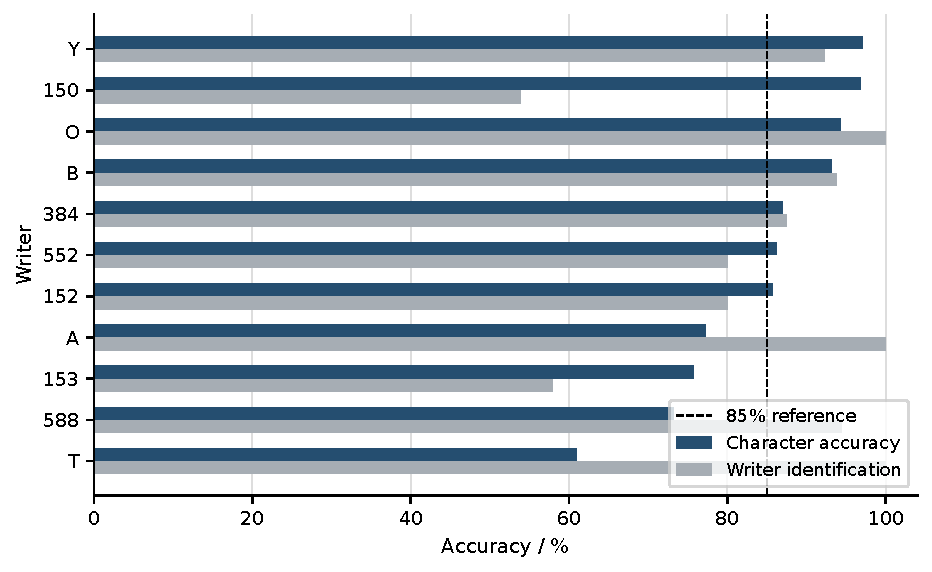
\includegraphics[width=0.98\linewidth]{Figures/results_writer_performance.pdf}
\caption{Physical reproduction by writer. Character accuracy and writer identification are measured separately. The dashed 85\% line is the character target and a visual reference for identification; identification does not replace the proposal's correlation criterion.}
\label{fig:res-writers}\end{figure}
\begin{figure}[!htbp]\centering
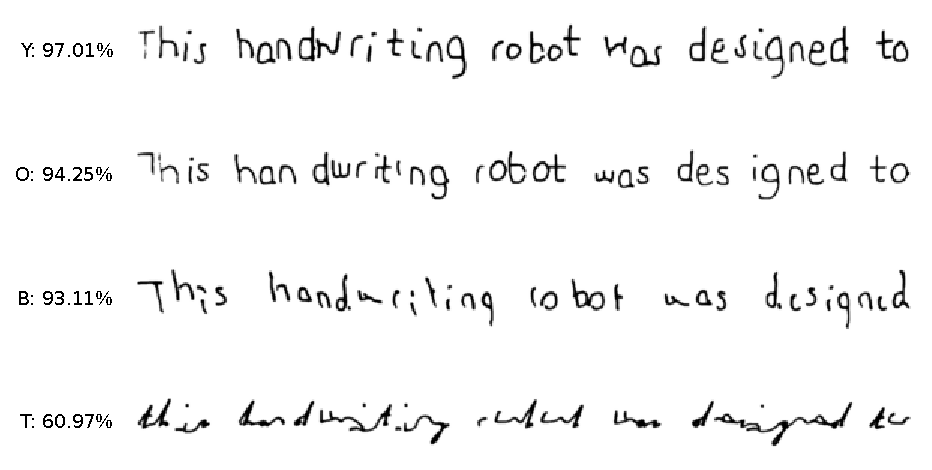
\includegraphics[width=0.98\linewidth]{Figures/results_physical_examples.pdf}
\caption{Stored crops from photographed robot pages for Y, O, B and T. The percentages label each writer's aggregate character score, not the accuracy of the single strip shown. These physical-output examples illustrate the range rather than constituting a new controlled same-sentence experiment.}
\label{fig:res-physical}\end{figure}

The automated reader recovers 84.41\% character accuracy overall, with 45.97\% positional word match. The writer is correctly identified on 159/184 lines (86.41\%), and all fourteen archived page pools are attributed correctly. Seven writers exceed 85\% character accuracy. Y, 150, O and B exceed 93\%, and Y, O, B and 384 exceed both 85\% character accuracy and 85\% line-level writer identification. These are demonstrated operating cases, rather than replacements for the pooled result.

The new physical style comparison applies the same fixed descriptor definitions to the 184 reproduced lines and 156 original validation lines, grouped by the eleven writers. All lines return usable descriptors and no writer is excluded. Original and reproduced text content is not matched sentence by sentence, so the comparison concerns writer-level geometry across these samples. Nine descriptors include pen-dependent ink density and stroke width; the seven shape descriptors omit those two quantities, consistently with the constant-pen design rationale.

Table~\ref{tab:res-physical-style} gives both variants. Standardising each feature across writers separately in the original and physical domains, then correlating the flattened arrays, gives 0.713 over all nine features and 0.697 over seven shape features. With original-domain statistics used for both arrays, the corresponding values are 0.633 and 0.611. Appendix~\ref{app:res-physical-style} gives the extraction and individual descriptors. This is a new retrospective measurement of saved physical output, not an extension of the earlier ten-writer synthetic experiment.
\begin{table}[!htbp]\centering\small
\begin{tabular}{lrrr}\toprule
\textbf{Feature set} & \textbf{Features} & \textbf{Separate domains} & \textbf{Absolute variant}\\\midrule
All geometric descriptors & 9 & 0.713 & 0.633\\
Shape descriptors (ink omitted) & 7 & 0.697 & 0.611\\
\bottomrule\end{tabular}
\caption{New physical-to-original comparison across eleven writers. The first correlation standardises features separately in each domain; the absolute variant uses original-domain statistics for both. The target reference is 0.85.}\label{tab:res-physical-style}
\end{table}


The physical slant coefficient is 0.991, ascender extent 0.817, character width 0.798 and word gap 0.486. For example, writer 150's mean estimated slant changes from $-5.17^\circ$ in the original reference lines to $-5.42^\circ$ in the physical output, approximately $-0.26^\circ$. Across equally weighted, separately standardised features, the pooled shape correlation is the mean of the seven per-feature correlations; their sum 4.8767 divided by seven gives 0.6967. It lies 0.1533 below the 0.85 reference.

\resstep{Observations}
The pooled character score is 0.59 percentage points below the 85\% target. Writer scores vary from 60.97\% to 97.01\%. The character score and writer-identification score do not rank writers identically: T is identified on every scored line while its character score is the lowest, and writer 150 has 96.75\% character accuracy with 53.85\% identification. Thus the two outputs measure different properties of reproduction.

The measured components-per-character descriptor of genuine handwriting is positively associated with reproduced character accuracy ($r=0.855$, Spearman $\rho=0.845$, eleven writers); a lower descriptor indicates more joined handwriting. The corresponding writer-identification rank association is $\rho=-0.027$. These are cross-writer associations, not measurements of the loss caused by an individual joining operation.

\resstep{Statistical analysis}
The descriptive Wilson interval on 159/184 identifications is 80.7--90.6\%. A 10\,000-repeat resampling of the eleven whole writer groups gives a central 95\% range of 77.82--90.27\% for pooled character accuracy. The new physical shape coefficient has a central writer-resampling range of 0.555--0.827. These ranges reflect sensitivity to which observed writers are represented. Shared texts, profiles and capture conditions limit an interpretation as independent generalisation trials. The final targets are assessed using the observed pooled scores and their breakdowns, without claiming a universal pass from the better individual cases.

\reportqt{qt:r2}{Reading handwritten content and identifying its writer (R2)}
\resstep{Objectives of the test or experiment}
Measure the two classification outputs against the 95\% target using data excluded from weight updates for the relevant network. The reader and writer model have different training populations, so their scores are reported separately rather than multiplied into an invented combined accuracy.

\resstep{Equipment used}
The saved IAM line corpus and photographed line crops; the evaluated scratch reader and joint-reader comparison; the 0.17-normalised eleven-writer model; and the transcript-scoring and per-line writer-classification tools on the development host. No gantry movement is required during this scoring stage.

\resstep{Test setup and experimental parameters}
The reader evaluation contains the distributor's 976 IAM validation lines (42\,072 characters) and 100 photographed validation lines (3\,675 characters). The latter use the recorded seeded 15\% line split. Transcript lookup found that many lines from IAM writers 150, 152 and 153 occur in the public training partition; their project-page scores are therefore not used as additional reader validation. The selected photographed and public validation sets are kept distinct. Validation data may have informed checkpoint selection, so these scores describe validation performance rather than a newly collected blind final test.

The writer evaluation contains 156 lines: a held-out labelled page for each of six database writers and the seeded photographed-line split. Photographed validation lines may share a writing session and page background with training lines. This is the split described in Section~\ref{sec:des-class}; its population is stated explicitly when interpreting the result.

\resstep{Steps followed in the test or experiment}
\begin{enumerate}\setlength{\itemsep}{1pt}
\item Check the reader evaluation transcripts against the public corpus partitions and retain the specified validation populations.
\item Read each validation line with greedy CTC decoding and retain the raw edit and reference counts.
\item Classify each writer-validation crop after the selected stroke normalisation; retain its reference, predicted class and confidence.
\item Aggregate by population and writer, and pool each writer's validation lines for the separate group-level result.
\end{enumerate}

\resstep{Results or measurements}
Table~\ref{tab:res-r2-reader} gives the reader scores. The scratch checkpoint yields 94.39\% pooled character accuracy, while the joint reader yields 94.06\% on the same population. The photographed subset yields 94.42\% with the scratch reader and 93.33\% with the joint reader. The author selects the library-trained joint reader for the demonstration. The comparison therefore supports the numerical implementation without substituting its result for the selected system.
\begin{table}[!htbp]\centering\small
\begin{tabular}{lrrrr}\toprule
\textbf{Evaluation set} & \textbf{Lines} & \textbf{Characters} & \textbf{Joint / \%} & \textbf{NumPy / \%}\\\midrule
Public IAM validation & 976 & 42072 & 94.12 & 94.39\\
Photographed A & 31 & 934 & 94.00 & 94.65\\
Photographed B & 19 & 739 & 95.81 & 97.70\\
Photographed O & 22 & 1017 & 94.40 & 94.79\\
Photographed T & 11 & 345 & 85.51 & 89.28\\
Photographed Y & 17 & 640 & 92.03 & 92.50\\
All & 1076 & 45747 & 94.06 & 94.39\\
\bottomrule\end{tabular}
\caption{Character accuracy of the selected library-trained joint reader and the evaluated NumPy-trained reader, using greedy CTC decoding. The public set is the distributor's validation partition, not an independent final test set.}\label{tab:res-r2-reader}
\end{table}


The library-trained writer model correctly classifies 153/156 lines, or 98.08\%. Pooling the available validation lines gives the correct identity for all eleven writers. The individual correct counts are 8/9, 7/8, 9/9, 12/12, 10/10 and 8/8 for the six database writers, and 31/31, 18/19, 22/22, 11/11 and 17/17 for A, B, O, T and Y. Figure~\ref{fig:res-holdout} gives the complete confusion matrix rather than only the overall percentage.
\begin{figure}[!htbp]\centering
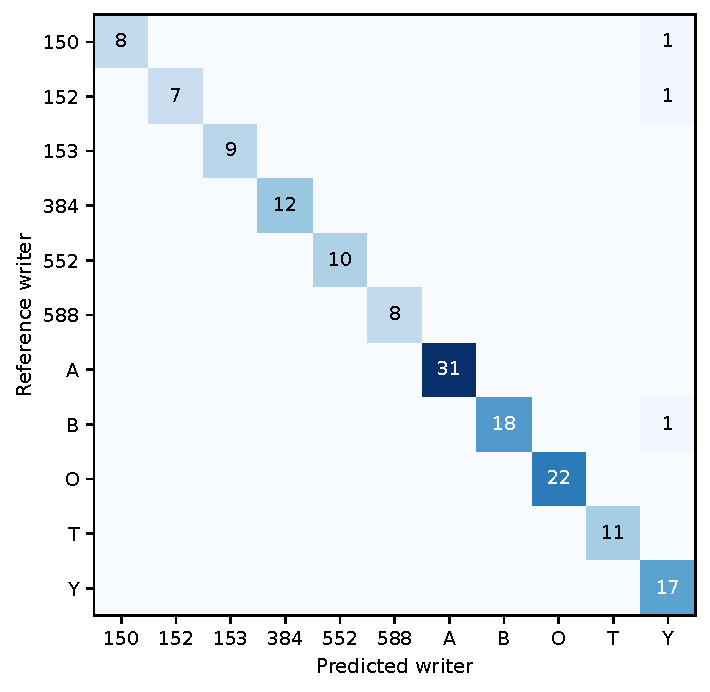
\includegraphics[width=0.84\linewidth]{Figures/results_holdout_confusion.pdf}
\caption{Writer classification on 156 validation lines. Rows are reference writers and columns are predicted writers; blank cells are zero. Three lines are misclassified, all as Y. Photographed writers use the seeded line split, while database writers use held-out pages.}
\label{fig:res-holdout}\end{figure}

\resstep{Observations}
The writer point estimate exceeds 95\% by 3.08 percentage points. The selected reader's pooled text score is 0.94 percentage points below 95\%; the strongest photographed writer's character score under the selected reader is 95.81\%. The selected reader gives 94.12\% on the public subset and 93.33\% on photographed lines, and recovers 221/1\,076 complete lines without an edit. The numerical reader's corresponding character scores are 94.39\% and 94.42\%, with 242 exact lines. The selected and numerical readers have pooled positional word-match scores of 72.16\% and 73.47\%, respectively.

The three writer errors have confidences of 44.2\%, 83.8\% and 39.5\%. Correct lines have mean confidence 97.7\%. The error with 83.8\% confidence shows that a high posterior is not a guarantee of correctness. The error indices are the last entries of their writer's evaluation group; this ordering alone does not establish a physical last-line or short-text cause for the randomly selected photographed subset.

\resstep{Statistical analysis}
The descriptive Wilson interval on writer accuracy is 94.5--99.3\%, and the interval on 11/11 correct writer pools is 74.1--100\%. The observed point estimates are strong, while the lower limits do not establish a population-wide 95\% guarantee. Treating all six predictions below 80\% confidence as wrong, in addition to the one higher-confidence error, leaves 149/156 correct (95.51\%); this is a sensitivity calculation on the same sample, not a measured rejection policy. For character accuracy, Equation~\ref{eq:res-char} is an edit ratio, so a binomial confidence interval on 45\,747 independent characters is not used.

\reportqt{qt:r3}{Complete reproduction time on the embedded platform (R3)}
\resstep{Objectives of the test or experiment}
Compare complete recorded reproduction times with the proposal allowance $4x$~s. The relevant operation includes generation and physical drawing, rather than physical motion alone.

\resstep{Equipment used}
The ODROID N2+, gantry and server stage timer. The primary measurement is the retained server log, including program-end and stop messages. No development-host inference benchmark supplies the physical timing result.

\resstep{Test setup and experimental parameters}
Generation and drawing use separate requests. The drawing request carries generation stages into its recorded reproduction total, as described by the job timing boundary in Section~\ref{sec:des-integration}. The primary analysis selects console records containing a drawing stage, a positive character count and an explicit successful program-end marker. Stopped jobs, zero-character commissioning shapes and unconfirmed summary-only entries are excluded from the pass count. Repeated records refer to recorded requests, not an assumed random sample of all possible text and styles.

\resstep{Steps followed in the test or experiment}
\begin{enumerate}\setlength{\itemsep}{1pt}
\item Associate a reproduction timer block with the preceding physical job's terminal status.
\item Retain explicitly completed positive-character jobs and read the recorded total and character count.
\item Calculate $t/x$ and compare $t$ with $4x$ for each retained record.
\item Group by text length and report the worst recorded total in each group.
\end{enumerate}

\resstep{Results or measurements}
Table~\ref{tab:res-r3-confirmed} and Figure~\ref{fig:res-r3} give 25 completion-confirmed records. Every retained total meets its numerical allowance. The largest normalised time is $166.61/43=3.8747$~s per character, leaving $172-166.61=5.39$~s on that request. At 378 characters the nine confirmed totals range from 507.57~s to 1\,085.01~s, against 1\,512~s allowed.
\begin{table}[!htbp]\centering\small
\begin{tabular}{rrrrr}\toprule
\textbf{Characters} & \textbf{Records} & \textbf{Allowance / s} & \textbf{Worst total / s} & \textbf{Worst / s per char}\\\midrule
43 & 9 & 172 & 166.61 & 3.875\\
75 & 1 & 300 & 188.60 & 2.515\\
82 & 3 & 328 & 260.33 & 3.175\\
91 & 2 & 364 & 222.63 & 2.446\\
132 & 1 & 528 & 277.90 & 2.105\\
378 & 9 & 1512 & 1085.01 & 2.870\\
\bottomrule\end{tabular}
\caption{ODROID reproduction records with explicit program-end confirmation. Generation and drawing are included in the recorded total. All 25 retained records meet their allowances.}\label{tab:res-r3-confirmed}
\end{table}


\resstep{Observations}
The shortest tested length has the narrowest worst-case margin: 3.1\% of its allowance. The longest tested paragraph has a worst-case margin of 28.2\%. The times for the same paragraph vary by a factor of 2.14. The log includes coordinate-clamping messages in some jobs, so completion of the interpreter and satisfaction of the timer do not by themselves prove that every intended trajectory remained unchanged. Character fidelity is assessed separately in QT~1.

\resstep{Statistical analysis}
All 25 confirmed records pass; their descriptive Wilson interval is 86.7--100\%. This is not a claim that future failure has been excluded. The experiment covers six observed lengths from 43 to 378 characters, with one to nine records per length. It provides no direct timing result for shorter requests or a probability of compliance across unseen styles.

\reportqt{qt:r4}{Time to decode a photographed page and identify its writer (R4)}
\resstep{Objectives of the test or experiment}
Compare the embedded classification request with $2+0.025x$~s and identify the time available for a practical improvement. Supporting acceleration experiments retain output checks alongside time measurements.

\resstep{Equipment used}
The ODROID server and stage timer for the two actual requests; the development host for the preserved comparison of sequential NumPy inference with batched PyTorch inference and for the image-resolution experiment. These are different timing platforms.

\resstep{Test setup and experimental parameters}
The ODROID log reports 500 characters over 16 lines and 982 characters over 22 lines. Their recorded totals include loading, conditioning, segmentation, cropping, reading and writer classification. Allowances below use the logged character counts; independent ground-truth counts and any acquisition latency outside the timer are not established by those records. The combined time is the pass criterion. Grouping image and network stages helps diagnose the overrun; it does not impose an additional independent specification on each group.

\resstep{Steps followed in the test or experiment}
\begin{enumerate}\setlength{\itemsep}{1pt}
\item Extract each recorded ODROID classification total and its component stages.
\item Compute the allowance from the recorded count and compare the total with it.
\item For the separate acceleration study, process the same stored pages with the same network weights and compare time and decoded text.
\item Repeat image preparation at half linear resolution, retaining line counts, failed pages and agreement with full-resolution output.
\end{enumerate}

\resstep{Results or measurements}
Table~\ref{tab:res-r4-times} and Figure~\ref{fig:res-r4} show the two ODROID requests. Neither meets R4: $46.26/14.50=3.19$ times the allowance and $55.49/26.55=2.09$ times the allowance. The network stages account for approximately 67.6\% of their combined time, and image stages 32.4\%.
\begin{table}[!htbp]\centering\small
\begin{tabular}{lrr}\toprule
\textbf{Recorded quantity} & \textbf{500 characters} & \textbf{982 characters}\\\midrule
Loading / s & 0.63 & 0.53\\
Conditioning / s & 6.61 & 6.04\\
Segmentation / s & 4.29 & 5.59\\
Cropping / s & 4.61 & 4.65\\
Image stages / s & 16.14 & 16.81\\
Reading / s & 19.02 & 24.66\\
Writer classification / s & 11.09 & 14.01\\
Network stages / s & 30.12 & 38.67\\
Total / s & 46.26 & 55.49\\
R4 allowance / s & 14.50 & 26.55\\
Overrun / s & 31.76 & 28.94\\
\bottomrule\end{tabular}
\caption{Two recorded ODROID classification requests. Totals are taken from the timer; rounded stage values may differ by 0.01 s when summed.}\label{tab:res-r4-times}
\end{table}


On fourteen stored pages, the development-host network experiment records 359.8~s for sequential NumPy inference and 130.3~s for equivalent library modules batched by page, a measured factor of 2.76. Decoded text agrees on every evaluated line. Both the execution backend and the batching strategy change together, so the factor cannot be assigned to batching alone. Writer-label equivalence is not established merely by identical reader text.

The image-resolution experiment finds 247 lines at full resolution and 182 at half resolution across the twelve pages that return results at both scales. None of those twelve retains its line count, and two additional reduced-resolution pages fail to return a segmentation. The reported 4.37-fold image-stage speed factor accompanies a mean text-agreement score of 33.8\%, so it is not an equivalent-output replacement. These comparisons are recorded in Appendix~\ref{app:res-speed}.

\resstep{Observations}
The observed network cost is 60.2 and 39.4~ms per logged character. Applying the host's 2.76-fold factor to those stage times would give 21.8 and 14.3~ms per character, respectively. These are useful design projections, not ODROID measurements. With unchanged image stages, even that projection gives totals of approximately 27.05~s and 30.82~s, still above the two allowances. A faster network path alone therefore does not close the demonstrated total-time gap under this projection.

\resstep{Statistical analysis}
Two ODROID requests establish two observed overruns; they do not establish a timing distribution or failure at every possible page length. The development-host comparison contains fourteen page conditions rather than repeated controlled ODROID runs. Its factor supports an optimisation candidate, while the embedded speed gain and complete R4 pass require direct measurement. A C or C++ implementation is not credited with an unmeasured speed-up.

\reportqt{qt:r5}{Gantry dimensional accuracy and geometric consistency (R5)}
\resstep{Objectives of the test or experiment}
Measure the drawn geometry relevant to the 0.5~mm positional target and distinguish dimensional checks from complete absolute-position and repeatability qualification.

\resstep{Equipment used}
The calibrated gantry, pen and paper; a metal non-digital vernier caliper, whose make, model and least count are not present in the retained record; and the generated 100~mm square and isosceles triangle of 80~mm base and nominal 40~mm height. The physical readings are author-recorded inputs, not outputs that can be regenerated by a script.

\resstep{Test setup and experimental parameters}
The retained measurements are from one square and one triangle after calibration. Four square sides and three triangle sides are compared with their commanded lengths. Caliper least count is not assumed from the number of digits typed in a result; reading uncertainty also depends on finite-width pen marks. The geometry provides a useful commissioning check for the coordinate and stepping model in Section~\ref{sec:des-drive}.

\resstep{Steps followed in the test or experiment}
\begin{enumerate}\setlength{\itemsep}{1pt}
\item Home and calibrate the gantry, then execute the square and triangle jobs.
\item Measure each reported side and calculate its difference from the nominal length.
\item Compare the dimensional differences with 0.5~mm and calculate the mean square-side error.
\item Use the unequal triangle sides to estimate an apparent apex offset under the stated geometric assumptions.
\end{enumerate}

\resstep{Results or measurements}
Table~\ref{tab:res-r5-lengths} retains all seven original readings. Figure~\ref{fig:res-geometry} shows their signed length errors. The four square sides have a mean absolute error of $(0.30+0.20+0.10+0.10)/4=0.175$~mm and maximum 0.30~mm. The largest absolute feature-length difference across both shapes is $|56.20-\sqrt{40^2+40^2}|=0.369$~mm.
\begin{table}[!htbp]\centering\small
\begin{tabular}{llrrr}\toprule
\textbf{Shape} & \textbf{Feature} & \textbf{Nominal / mm} & \textbf{Measured / mm} & \textbf{Error / mm}\\\midrule
Square & Bottom X & 100.00 & 100.30 & +0.30\\
Square & Top X & 100.00 & 100.20 & +0.20\\
Square & Left Y & 100.00 & 100.10 & +0.10\\
Square & Right Y & 100.00 & 99.90 & -0.10\\
Triangle & Base & 80.00 & 80.30 & +0.30\\
Triangle & Left slope & 56.57 & 56.20 & -0.37\\
Triangle & Right slope & 56.57 & 56.90 & +0.33\\
\bottomrule\end{tabular}
\caption{Author-recorded dimensions from one calibrated square and one triangle. These are feature-length errors, rather than an absolute coordinate-error map.}\label{tab:res-r5-lengths}
\end{table}


Place the measured base endpoints at $(-b/2,0)$ and $(b/2,0)$ and the apex at $(d,h)$. Subtracting the two squared-distance equations gives the project's geometric diagnostic:
\begin{equation}
d=\frac{\ell^2-r^2}{2b},\qquad \phi_{\rm app}=\arctan(d/h).
\label{eq:res-apex}
\end{equation}
Using $b=80.30$~mm, $\ell=56.20$~mm, $r=56.90$~mm and the nominal $h=40$~mm gives $d=-0.493$~mm and $\phi_{\rm app}=-0.706^\circ$. The angle is conditional on the assumed height and a shear interpretation; it is not an independent measurement of rail squareness. Both an ideal square and a rhombus can have equal side lengths, which is why diagonal or coordinate measurements would add information absent from the square-side test.

\resstep{Observations}
Every measured feature length is within 0.5~mm of nominal. The two horizontal square sides are long by 0.20--0.30~mm, while the vertical sides straddle nominal by 0.10~mm. The unequal sloping triangle sides are consistent with lateral geometric asymmetry. The measurements do not isolate scale, shear, pen width and reading uncertainty into separate physical causes.

\resstep{Statistical analysis}
There is one specimen of each shape. The spread among sides is not repeated-draw variability, and no standard deviation of repeatability is assigned. Side lengths alone also leave a rigid translation undetected, so the 0.5~mm absolute point-position requirement is not fully proven. The positive result is a dimensional error below the numerical limit on every measured feature; repeated word overlays and bed-coordinate measurements would complete the distinction requested in the proposal.

\reportqt{qt:r6}{Storage and use of multiple trained styles (R6)}
\resstep{Objectives of the test or experiment}
Confirm at least ten represented writers, stored glyph mappings and the ability to use those mappings for reproduction.
\resstep{Equipment used}
The evaluated eleven-class writer checkpoint, stored style profiles and glyph libraries, saved generated jobs and fourteen physical output pages.
\resstep{Test setup and experimental parameters}
The required count is ten. The evaluated set is 150, 152, 153, 384, 552, 588, A, B, O, T and Y. Both class identities and stored trajectory libraries are checked.
\resstep{Steps followed in the test or experiment}
Compare the classifier mapping with the stored profiles, then confirm that every identity occurs in the writer-validation records, physical pages and generated jobs.
\resstep{Results or measurements}
Eleven identities have classifier entries and stored profiles. All have physical samples in Figure~\ref{fig:res-writers} and correct pooled identities in QT~2, exceeding the required count by one.
\resstep{Observations}
The result demonstrates concurrent use of multiple stored styles; QT~1 measures their different reproduction quality.
\resstep{Statistical analysis}
This is an inventory count, so a sampling interval is inapplicable. R6 is met by the evaluated eleven-style set.

\subsubsection{Qualification under the proposal's field conditions}
\label{sec:res-conditions}
Indoor captures and physical drawings demonstrate operation in the fixed test arrangement. The author reports successful operation across lighting conditions wider than the planned range, but no illuminance readings or surface-level/vibration measurements accompany the retained records. The evidence supports the observed bench conditions and capture examples in Section~\ref{sec:des-segverify}; it does not numerically establish the 400--1000~lux endpoints. Table~\ref{tab:res-summary} compares the retained evidence with the proposal's exact environmental conditions.
\FloatBarrier
